\section{The MSL Radiation Assessment Detector}
\label{sec:mslrad}

\begin{figure}
    \centering
    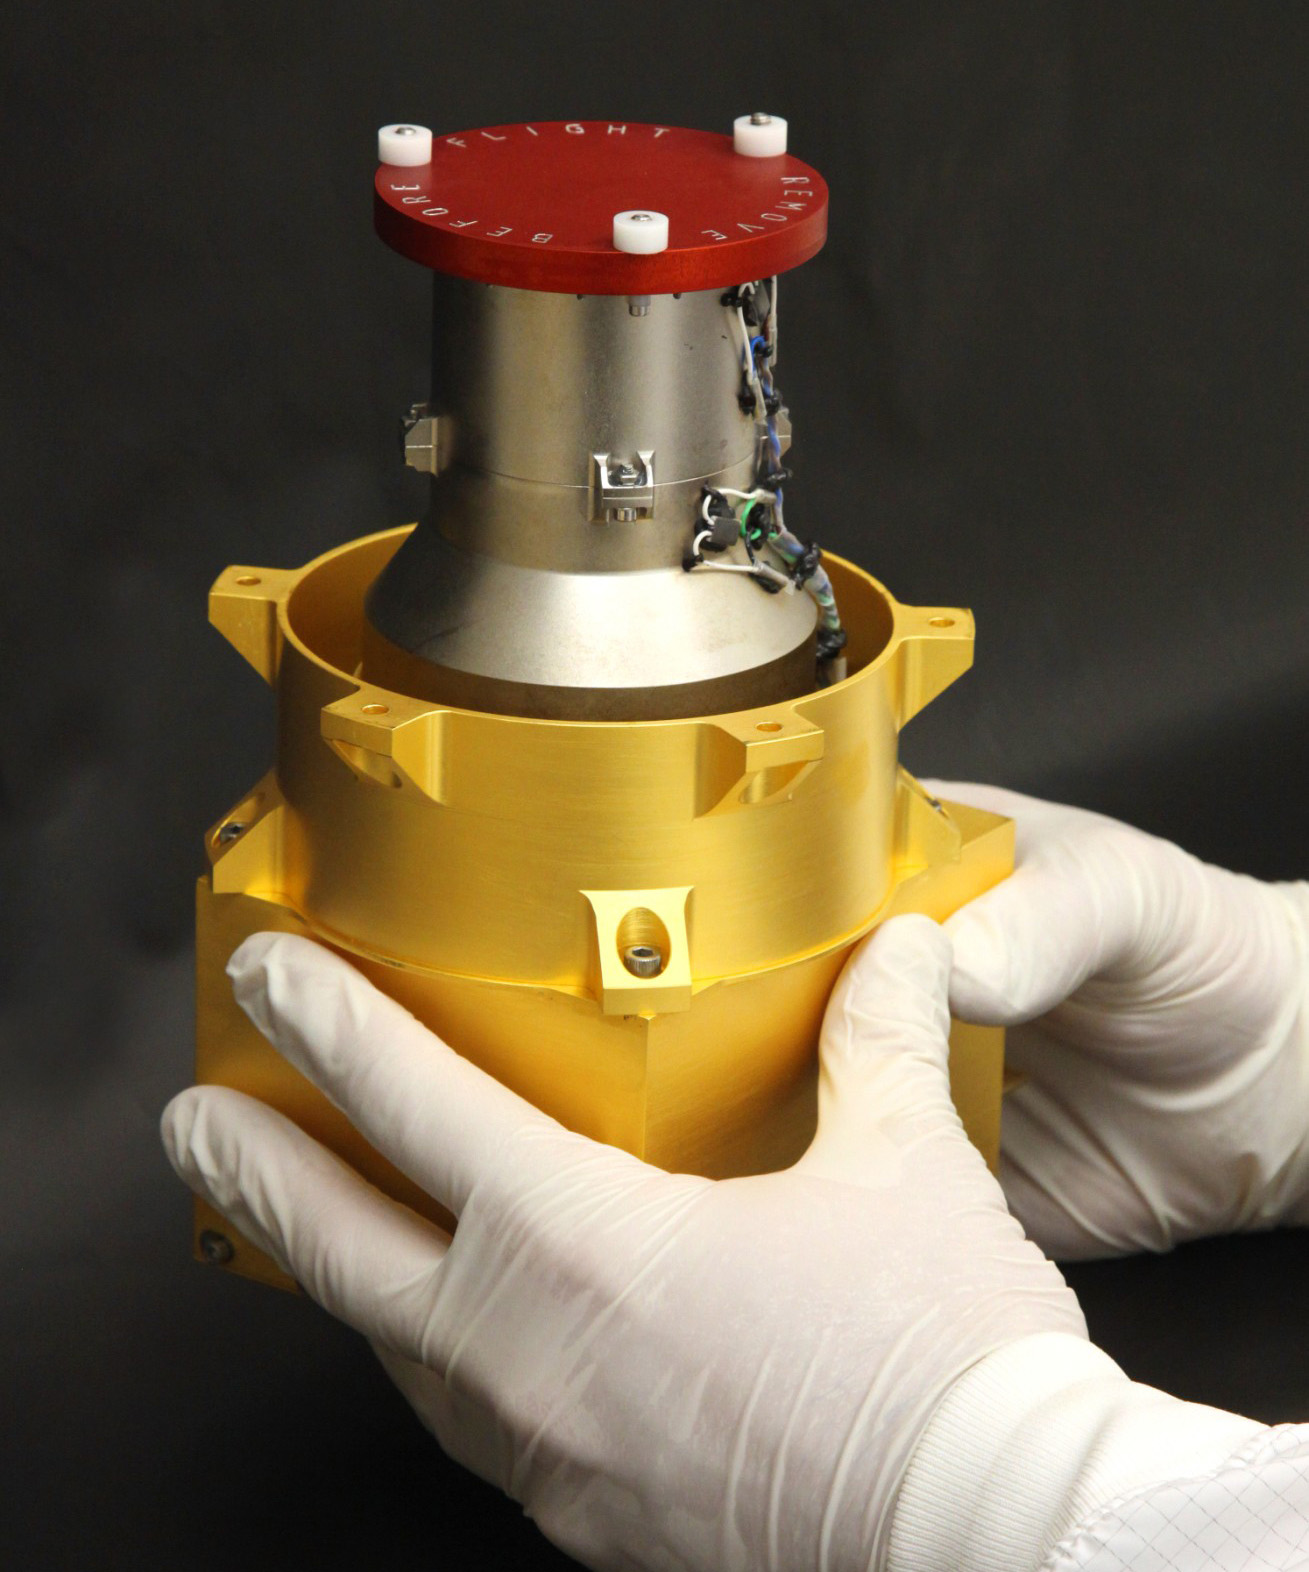
\includegraphics[width=0.4\linewidth]{images/rad}
    \caption[Photo of the \acs{RAD} sensor head]{A photo of the \ac{RAD} sensor head before it was mounted on the \ac{MSL} spacecraft. Source: NASA/JPL-Caltech/SwRI}
    \label{subfig:rad-photo}
\end{figure}


\begin{figure}
    \centering
    %\documentclass{standalone}
%\usepackage{tikz}
%\usepackage{amsmath}

%\usetikzlibrary{calc}
%\usetikzlibrary{decorations.pathmorphing}

%\definecolor{light-gray}{gray}{0.9}

%\begin{document}
\begin{tikzpicture}[scale=0.8]
    \tikzset{%
        add/.style args={#1 and #2}{
            to path={%
                ($(\tikztostart)!-#1!(\tikztotarget)$)--($(\tikztotarget)!-#2!(\tikztostart)$)%
                \tikztonodes},add/.default={.2 and .2}}
    }  
    
    \def\bottomwidth{3.25}
    \def\midwidth{1.8}
    \def\topwidth{1.65}
    \def\bottomheight{2.5}
    \def\midheight{4.375}
    \def\Fthickness{1}
    \def\Sithickness{0.1}
    \def\BCdistance{0.15}
    \def\topheight{8.375}
    
    % FOV
    \draw[add=0 and 0.3, dashed] (\midwidth - \Fthickness, \midheight) to (-\topwidth, \topheight);
    \draw[add=0 and 0.3, dashed] (-\midwidth + \Fthickness, \midheight) to (\topwidth, \topheight);

    % A
    \draw[fill=light-gray] (-\topwidth, \topheight - \Sithickness) rectangle (\topwidth, \topheight);
    \draw (-\midwidth + \Fthickness, \topheight - \Sithickness) --  (-\midwidth + \Fthickness, \topheight);
    \draw (-\midwidth + \Fthickness, \topheight - \Sithickness) --  (-\midwidth + \Fthickness, \topheight);
    \draw (\midwidth - \Fthickness, \topheight - \Sithickness) --  (\midwidth - \Fthickness, \topheight);
    \draw (\midwidth - \Fthickness, \topheight - \Sithickness) --  (\midwidth - \Fthickness, \topheight);
    \draw[latex-] (-\topwidth, \topheight - \Sithickness / 2) -- (-\topwidth - 0.5, \topheight - \Sithickness / 2) node[left] {A};
    
    % B
    \draw[fill=light-gray] (-\topwidth, \midheight + \BCdistance) rectangle (\topwidth, \midheight + \BCdistance + \Sithickness);
    \draw (-\midwidth + \Fthickness, \midheight + \BCdistance) --  (-\midwidth + \Fthickness, \midheight + \BCdistance + \Sithickness);
    \draw (-\midwidth + \Fthickness, \midheight + \BCdistance) --  (-\midwidth + \Fthickness, \midheight + \BCdistance + \Sithickness);
    \draw (\midwidth - \Fthickness, \midheight + \BCdistance) --  (\midwidth - \Fthickness, \midheight + \BCdistance + \Sithickness);
    \draw (\midwidth - \Fthickness, \midheight + \BCdistance) --  (\midwidth - \Fthickness, \midheight + \BCdistance + \Sithickness);
    \draw[latex-] (-\topwidth, \midheight + \BCdistance + \Sithickness / 2) -- (-\topwidth - 0.5, \midheight + \BCdistance + \Sithickness / 2 + 0.3) node[left] {B};
    
    % C
    \draw[fill=light-gray] (-\topwidth, \midheight) rectangle (\topwidth, \midheight + \Sithickness);
    \draw (-\midwidth + \Fthickness, \midheight) --  (-\midwidth + \Fthickness, \midheight + \Sithickness);
    \draw (-\midwidth + \Fthickness, \midheight) --  (-\midwidth + \Fthickness, \midheight + \Sithickness);
    \draw (\midwidth - \Fthickness, \midheight) --  (\midwidth - \Fthickness, \midheight + \Sithickness);
    \draw (\midwidth - \Fthickness, \midheight) --  (\midwidth - \Fthickness, \midheight + \Sithickness);
    \draw[latex-] (-\topwidth, \midheight + \Sithickness / 2) -- (-\topwidth - 0.5, \midheight + \Sithickness / 2) node[left] {C};
    
    % border of ABC
    \draw (-\topwidth, \midheight) -- (-\topwidth, \topheight);
    \draw (\topwidth, \midheight) -- (\topwidth, \topheight);
    
    % D
    \draw[fill=light-gray] (\bottomwidth - \Fthickness, \bottomheight) --  (-\bottomwidth + \Fthickness, \bottomheight) -- (-\midwidth + \Fthickness, \midheight) -- (\midwidth - \Fthickness, \midheight) -- (\bottomwidth - \Fthickness, \bottomheight);   
    \node at (0, {\bottomheight + (\midheight - \bottomheight) / 2}) {D};   
    
    % E
    \draw[fill=green!50] (\bottomwidth - \Fthickness, \bottomheight) -- (\bottomwidth - \Fthickness, \Fthickness) --
    (-\bottomwidth + \Fthickness, \Fthickness) --  (-\bottomwidth + \Fthickness, \bottomheight) -- (\bottomwidth - \Fthickness, \bottomheight);  
    \node at (0, {\Fthickness + (\bottomheight - \Fthickness) * 0.4}) {E};   
    
    % F
    \draw[fill=yellow] (-\bottomwidth, 0) -- (\bottomwidth, 0) -- (\bottomwidth, \bottomheight) -- (\midwidth, \midheight) --
    (\midwidth - \Fthickness, \midheight) -- (\bottomwidth - \Fthickness, \bottomheight) -- (\bottomwidth - \Fthickness, \Fthickness) --
    (-\bottomwidth + \Fthickness, \Fthickness) --  (-\bottomwidth + \Fthickness, \bottomheight) -- (-\midwidth + \Fthickness, \midheight) --
    (-\midwidth, \midheight) -- (-\bottomwidth, \bottomheight) -- (-\bottomwidth, 0);     
    \node at (0, \Fthickness / 2) {F};
    
    % trajectories of ions
    \draw[thick, green, -latex] (-\topwidth*0.7, \topheight*1.15) node[above, align=center] {\small Ion\\ \small (accepted)}
     -- ({-(\midwidth - \Fthickness) * 0.5}, \midheight + \Sithickness / 2);
    \draw[thick, green, -latex] (\topwidth*0.65, \topheight*1.15) node[above, align=center] {\small Ion\\ \small (accepted)}
     -- ({-(\midwidth - \Fthickness) * 0.5}, {\bottomheight +  (\midheight - \bottomheight) / 2});
    \draw[thick, red, -latex] (0, \topheight*1.3) node[above, align=center] {\small Ion\\ \small (rejected)}
     -- (0, \topheight - \Sithickness / 2);
    \draw[thick, red, -latex] (\bottomwidth, \midheight) node[above right, align=center] {\small Ion\\ \small (rejected)}
    -- (\bottomwidth * 0.4, {\bottomheight + (\midheight - \bottomheight) * 0.2});
    
    % trajectory of neutron
    \draw[thick, gray, -latex] (-\bottomwidth*0.3, -0.5) node[below] {\small Neutron (accepted)}
    -- (-\bottomwidth*0.3, {\Fthickness + \bottomheight * 0.2});
    \draw[thick, gray, -latex]  (-\bottomwidth*0.3, {\Fthickness + \bottomheight * 0.2}) -- (-\bottomwidth * 1.1, \bottomheight * 1.3);
    \draw[thick, blue, -latex]  (-\bottomwidth*0.3, {\Fthickness + \bottomheight * 0.2}) -- (0, \bottomheight * 1.1) node[midway, right, xshift=1mm] {\small Recoil proton};
    
    % trajectory of gamma
    \draw[thick, gray, decorate, decoration=snake] (-\bottomwidth*1.2, \bottomheight * 0.8) node[below, align=center, xshift=-4mm] {\small $\gamma$-ray\\ \small (accepted)} -- (-\bottomwidth * 0.3, \bottomheight * 1.4);
    \draw[thick, gray, -latex] (-\bottomwidth * 0.3, \bottomheight * 1.4) -- ++ (\bottomwidth * 0.03, \bottomheight * 0.02);
    
\end{tikzpicture}
%\end{document}
    \caption[Schematic diagram of the \acs{RAD} sensor head]{Schematic diagram of the \ac{RAD} sensor head. Red, green and gray arrows show possible trajectories of charged and neutral particles through the detectors. Based on      \textcite{Hassler-2012-MSLRAD}, Fig. 7b}
    \label{fig:rad-sensorhead}
\end{figure}


\section{The Solar Orbiter High Energy Telescope}
\label{sec:solohet}

\section{Neutron monitor measurements}
\label{sec:neutronmonitors}

\section{The STEREO Heliospheric Imagers}
\label{sec:stereohi}

\begin{figure}
    \centering
    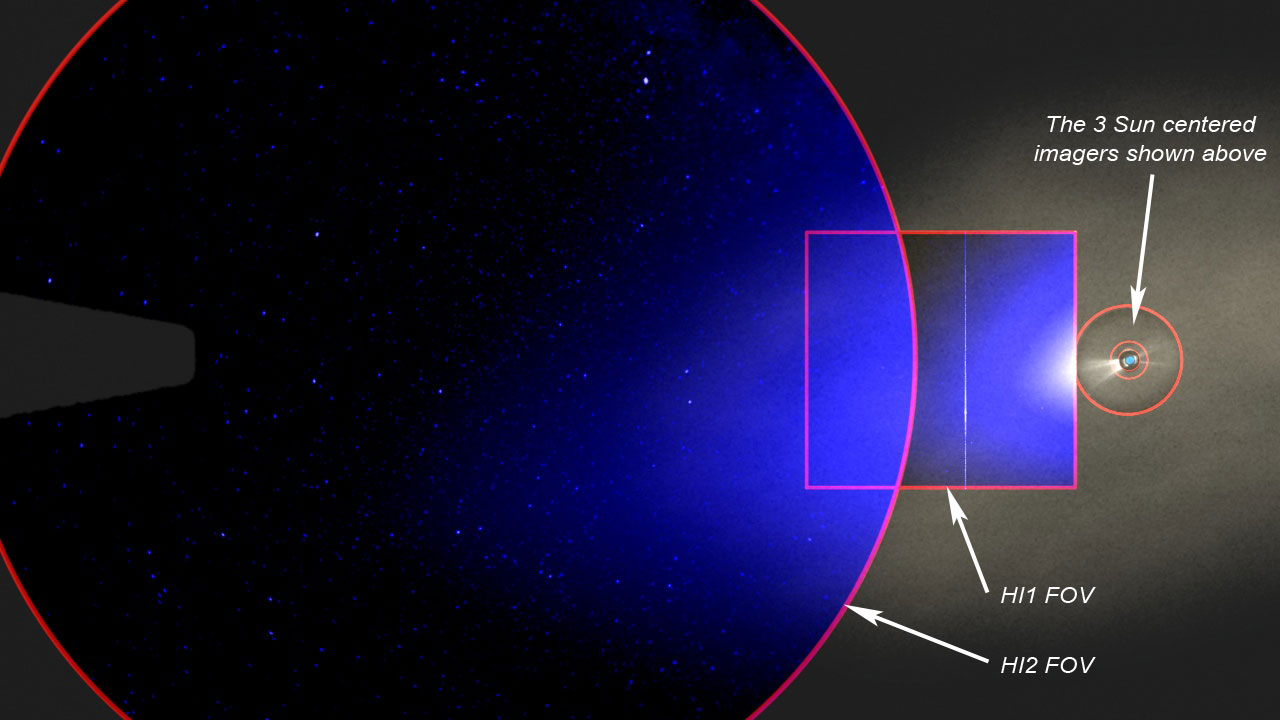
\includegraphics[width=0.8\linewidth]{images/secchi_fov}
    \caption[Fields of view of the \acs{STEREO} SECCHI telescopes]{Fields of view of the \ac{STEREO} SECCHI telescopes EUVI, COR1, COR2 (circles on the right side), and HI1 and HI2. Source: NASA/STEREO/GSFC}
    \label{fig:secchifov}
\end{figure}
